\documentclass[a4paper,10pt,fleqn]{article}

\usepackage{layout}

\begin{document}

\subsubsection*{Bezeichnung des LZI-Übertragungsgliedes}
\[ PT_2 \]

\subsubsection*{Übertragungsfunktion $G(s)$}
\[ \frac{4}{3 s^2 + 2 s + 1} \]

\subsubsection*{Stabilität des Übertragungsgliedes (Pole, Nulstellen, Plan)}
Nullstellen: keine, da $s$ im Zähler nicht vorkommt. \\\\
Polstellen: 
\[ 3 s^2 + 2 s + 1 = \left(s + \frac{1}{3} - \frac{\sqrt{2}}{3}j\right) \cdot \left(s + \frac{1}{3} + \frac{\sqrt{2}}{3}j\right) \]
\[ \rightarrow s_1 = -\frac{1}{3} + \frac{\sqrt{2}}{3}j \qquad s_2 = -\frac{1}{3} - \frac{\sqrt{2}}{3}j \]
\begin{figure}[h!]
    \centering
    \begin{tikzpicture}[scale=4,domain=-1.1:1.1]
        \draw [->] (-1.1,0) -- (1.1,0) node[below] {$Re$};
        \draw [->] (0,-1.1) -- (0,1.1) node[left]  {$Im$};

        \draw [-] (-1,0.02) -- (-1,-0.02) node[below] {$-1$};
        \draw [-] (1,0.02) -- (1,-0.02) node[below] {$-1$};
        \draw [-] (0.02,-1) -- (-0.02,-1) node[right] {$-1$};
        \draw [-] (0.021,1) -- (-0.02,1) node[right] {$-1$};

        \fill [red] (-1/3, 2^0.5/3) circle (.5pt) node [above,black] {$s_1 = -\frac{1}{3} + \frac{\sqrt{2}}{3}j$};
        \fill [red] (-1/3,-2^0.5/3) circle (.5pt) node [above,black] {$s_2 = -\frac{1}{3} - \frac{\sqrt{2}}{3}j$};
    \end{tikzpicture}
\end{figure}

\subsubsection*{Zugehörige Differentialgleichung}
\[ \frac{4}{3 s^2 + 2 s + 1} = G(s) = \frac{V(s)}{U(s)} \]
\[ 4 U(s) = 3 s^2 V(s) + 2 s V(s) + V(s) \]
\[ 4 u(t) = 3 \ddot{v}(t) + 2 \dot{v}(t) + v(t) \]
\[ \frac{3}{4} \ddot{v}(t) + \frac{1}{2} \dot{v}(t) + v(t) = u(t) \]

\subsubsection*{Berechnung der Einheitssprungantwort (Übertragungsfunktion) ($G(s)$, $H(s)$, $PBZ$, $L^-1$, $h(t)$, Skizze)}
\[ Y(s) = \frac{4 \cdot G(s)}{3 s^2 + 2 s + 1} \]
\[ Y(s) = \frac{4 \cdot \frac{1}{s}}{3 s^2 + 2 s + 1} = \frac{4}{s \cdot (3 s^2 + 2 s + 1)} \]
\[ \frac{A}{s} + \frac{C_1 s + C_2}{3 s^2 + 2 s + 1} = \frac{4}{s \cdot (3 s^2 + 2 s + 1)} \]
\[ A \cdot (3 s^2 + 2 s + 1) + C_1 \cdot s^2 + C_2 \cdot s = 4 \]
\[ 3 A + C_1 = 0 \]
\[ 2 A + C_2 = 0 \]
\[ A = 4 \]
\[ C_1 = -12 \]
\[ C_2 = -8 \]
\[ \frac{4}{s} - \frac{12 s}{3 s^2 + 2 s + 1} - \frac{8}{3 s^2 + 2 s + 1} 
= \frac{4}{s} - 4 \cdot \frac{s}{s^2 + \frac{2}{3} s + \frac{1}{3}} - \frac{8}{3} \cdot \frac{1}{s^2 + \frac{2}{3} s + \frac{1}{3}} \]

\subsubsection*{Berechnung und Skizze des Bode-Diagramms ($G(j\omega)$, $|G(j\omega)|_{dB}$, $arc(G(j\omega))$)}
\[ K = 4 \Rightarrow 20 \cdot \log_{10}(4) = 12.04 \]
\begin{figure}[h!]
    \centering
    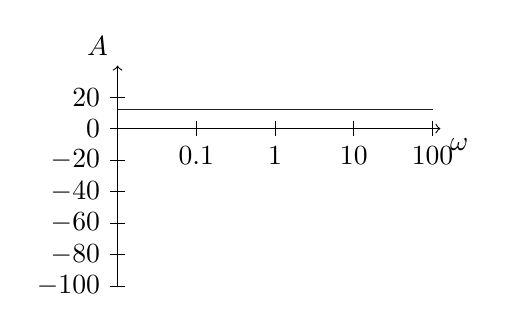
\begin{tikzpicture}[xscale=0.1, yscale=0.02, domain=0:41]
        \draw [->] (0,0) -- (41,0) node[below right] {$\omega$};
        \draw [->] (0,-100) -- (0,40) node[above left] {$A$};

        \draw (10,5) -- (10,-5) node[below] {$0.1$};
        \draw (20,5) -- (20,-5) node[below] {$1$};
        \draw (30,5) -- (30,-5) node[below] {$10$};
        \draw (40,5) -- (40,-5) node[below] {$100$};
        \draw (1,20) -- (-1,20) node[left] {$20$};
        \draw (1,0) -- (-1,0) node[left] {$0$};
        \draw (1,-20) -- (-1,-20) node[left] {$-20$};
        \draw (1,-40) -- (-1,-40) node[left] {$-40$};
        \draw (1,-60) -- (-1,-60) node[left] {$-60$};
        \draw (1,-80) -- (-1,-80) node[left] {$-80$};
        \draw (1,-100) -- (-1,-100) node[left] {$-100$};

        \draw [blue] (0,12.4) -- (40,12.4);
    \end{tikzpicture}
    \begin{tikzpicture}[xscale=0.1, yscale=0.015, domain=0:41]
        \draw [->] (0,0) -- (41,0) node[below right] {$\omega$};
        \draw [->] (0,-180) -- (0,10) node[above left] {$\varphi$};

        \draw (10,5) -- (10,-5) node[below] {$0.1$};
        \draw (20,5) -- (20,-5) node[below] {$1$};
        \draw (30,5) -- (30,-5) node[below] {$10$};
        \draw (40,5) -- (40,-5) node[below] {$100$};
        \draw (1,0) -- (-1,0) node[left] {$0$};
        \draw (1,-45) -- (-1,-45) node[left] {$-45$};
        \draw (1,-90) -- (-1,-90) node[left] {$-90$};
        \draw (1,-135) -- (-1,-135) node[left] {$-135$};
        \draw (1,-180) -- (-1,-180) node[left] {$-180$};

        \draw [blue] (0,0) -- (40,0);
    \end{tikzpicture}
\end{figure}

\[ 3 s^2 + 2 s + 1 \]
\begin{figure}[h!]
    \centering
    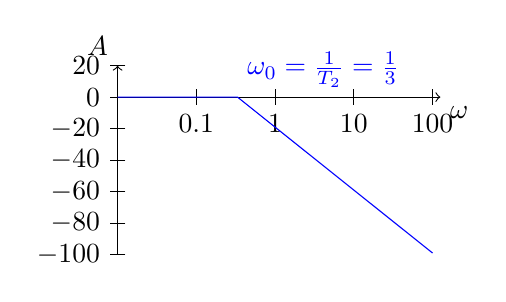
\begin{tikzpicture}[xscale=0.1, yscale=0.02, domain=0:41]
        \draw [->] (0,0) -- (41,0) node[below right] {$\omega$};
        \draw [->] (0,-100) -- (0,20) node[above left] {$A$};

        \draw (10,5) -- (10,-5) node[below] {$0.1$};
        \draw (20,5) -- (20,-5) node[below] {$1$};
        \draw (30,5) -- (30,-5) node[below] {$10$};
        \draw (40,5) -- (40,-5) node[below] {$100$};
        \draw (1,20) -- (-1,20) node[left] {$20$};
        \draw (1,0) -- (-1,0) node[left] {$0$};
        \draw (1,-20) -- (-1,-20) node[left] {$-20$};
        \draw (1,-40) -- (-1,-40) node[left] {$-40$};
        \draw (1,-60) -- (-1,-60) node[left] {$-60$};
        \draw (1,-80) -- (-1,-80) node[left] {$-80$};
        \draw (1,-100) -- (-1,-100) node[left] {$-100$};

        \draw [blue] (0,0) -- (15.23,0) node[above right] {$\omega_0 = \frac{1}{T_2} = \frac{1}{3}$} -- (40,-99);
    \end{tikzpicture}
    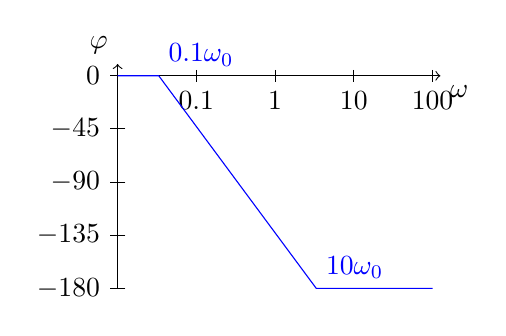
\begin{tikzpicture}[xscale=0.1, yscale=0.015, domain=0:41]
        \draw [->] (0,0) -- (41,0) node[below right] {$\omega$};
        \draw [->] (0,-180) -- (0,10) node[above left] {$\varphi$};

        \draw (10,5) -- (10,-5) node[below] {$0.1$};
        \draw (20,5) -- (20,-5) node[below] {$1$};
        \draw (30,5) -- (30,-5) node[below] {$10$};
        \draw (40,5) -- (40,-5) node[below] {$100$};
        \draw (1,0) -- (-1,0) node[left] {$0$};
        \draw (1,-45) -- (-1,-45) node[left] {$-45$};
        \draw (1,-90) -- (-1,-90) node[left] {$-90$};
        \draw (1,-135) -- (-1,-135) node[left] {$-135$};
        \draw (1,-180) -- (-1,-180) node[left] {$-180$};

        \draw [blue] (0,0) -- (5.23,0) node[above right] {$0.1 \omega_0$} -- (25.23,-180) node[above right] {$10 \omega_0$} -- (40,-180);
    \end{tikzpicture}
\end{figure}

\begin{figure}[h!]
\center
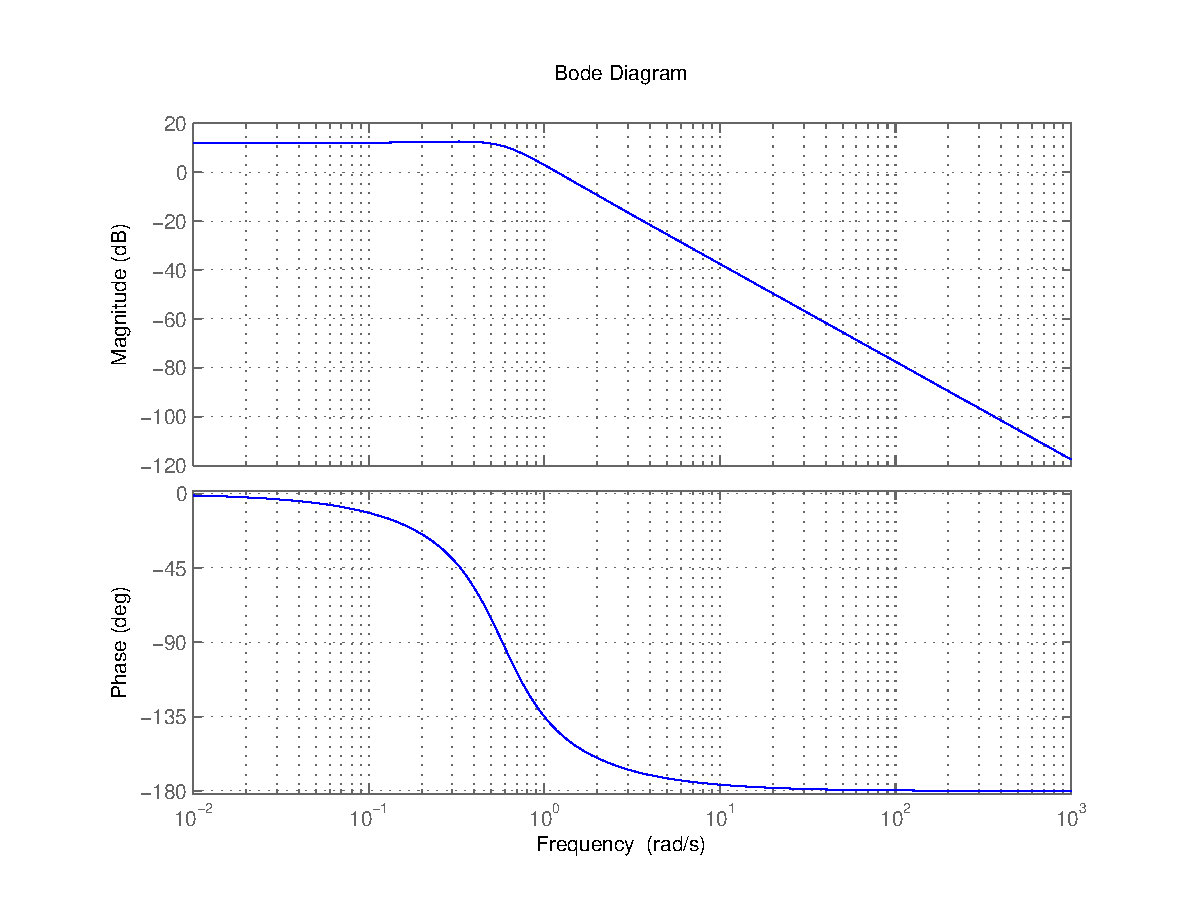
\includegraphics[width=\textwidth]{bode.eps}
\end{figure}

\subsubsection*{Skizze der Nyquist Ortskurve ($G(j\omega)$)}
\[ \frac{4}{3(j\omega)^2 + 2(j\omega) + 1} = \frac{4}{-3 \omega^2 + 2 j \omega + 1} 
= \frac{4 (-3 \omega^2 - 2 j \omega + 1)}{9 \omega^4 - 2 \omega^2  + 1} \]
\[ = \frac{-12 \omega^2 + 4}{9 \omega^4 - 2 \omega^2 + 1} - \frac{8 \omega}{9 \omega^4 - 2 \omega^2 + 1}j \]
Realteil: 
\[  \frac{-12 \omega^2 + 4}{9 \omega^4 - 2 \omega^2 + 1} \]
Imaginärteil: 
\[ - \frac{8 \omega}{9 \omega^4 - 2 \omega^2 + 1} \]
\begin{figure}[h!]
\center
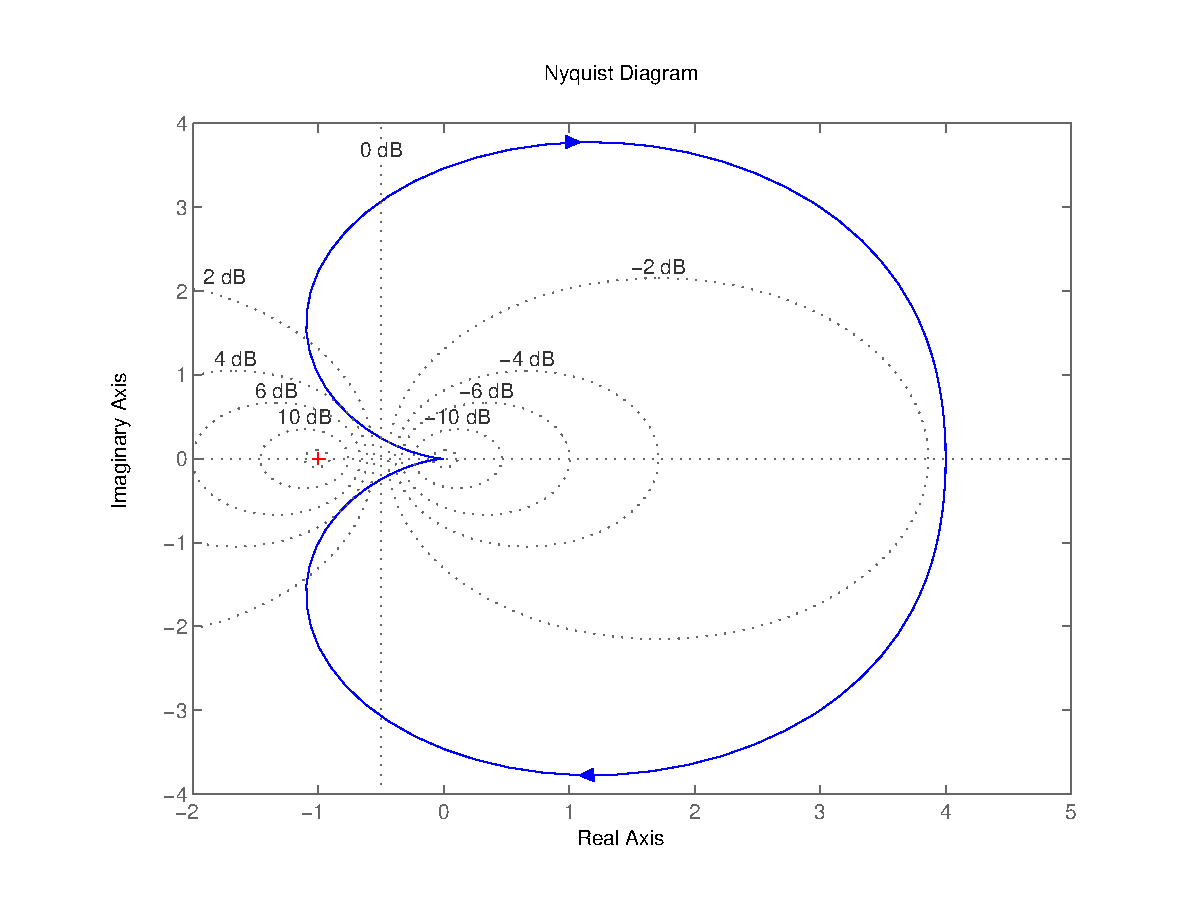
\includegraphics[width=\textwidth]{nyquist.eps}
\end{figure}

\end{document}
